\begin{figure}[t]
\centering
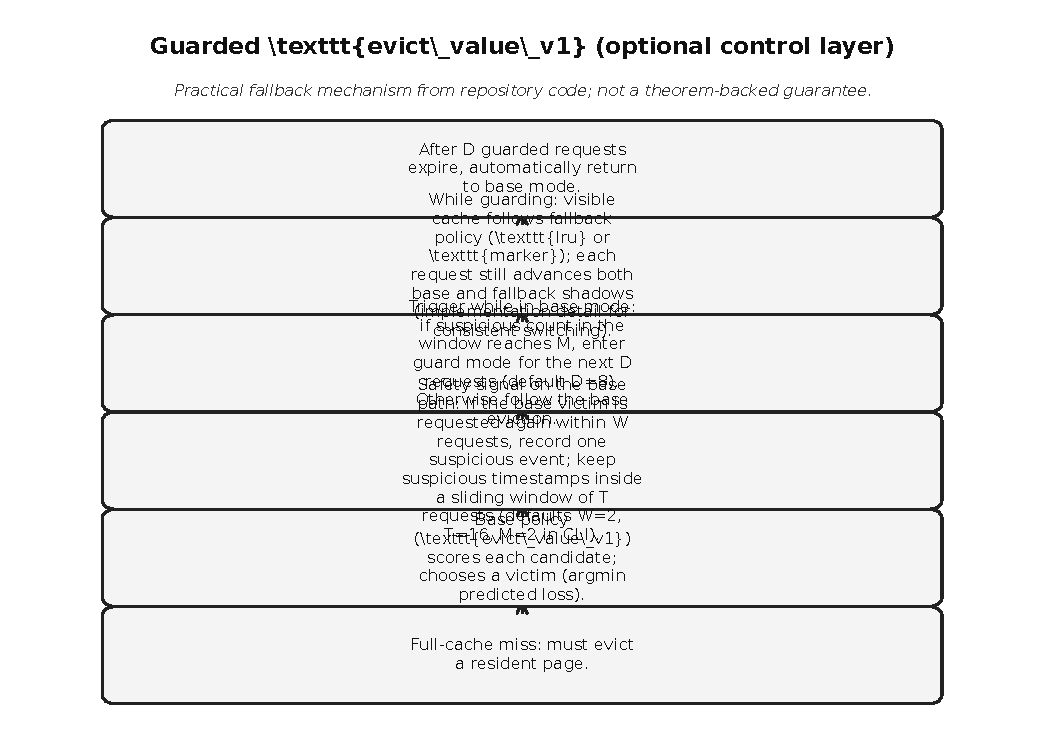
\includegraphics[width=\columnwidth]{figures/manuscript/figure6_guard_wrapper_evict_value_v1.pdf}
\caption{Optional guard wrapper (\texttt{evict\_value\_v1\_guarded}). On full-cache misses the base learned policy scores residents. A lightweight \emph{early-return} detector tracks whether the base victim is quickly re-requested; suspicious events in a bounded time window can trigger a fixed-duration fallback to \texttt{lru} or \texttt{marker}. Both policies are stepped each request for consistent shadow state (see \path{src/lafc/policies/guard_wrapper.py}). This is an empirical control layer described in-repository; it is not asserted as a competitive robustness theorem.}
\label{fig:guard-wrapper-evict-value-v1}
\end{figure}
